\documentclass[withoutpreface,bwprint]{cumcmthesis} %去掉封面与编号页
\usepackage[final]{pdfpages}
\title{《软件需求工程 B》 大作业课题}
\tihao{A}

\baominghao{4321}
\schoolname{武汉理工大学}
\membera{小米}
\memberb{向左}
\memberc{哈哈}
\supervisor{老师}
\yearinput{2017}
\monthinput{08}
\dayinput{22}

% 添加pdf封面
% \usepackage[final]{pdfpages}
% 
\includepdf[pages={1,2}]{head.pdf}
% \newpage


% \begin{enumerate}[itemindent=1em]  %在这里设置缩进的距离
%     \item 将信号量S的值减1,即进行S = S-1;   
% \end{enumerate}

% \newpage
% % 代码附录
% \begin{appendices}
% \section{爬取店铺POI}
% \begin{lstlisting}[language=python]
%  \end{lstlisting}
% \section{评论数据爬取}
% \begin{lstlisting}[language=python]
% \end{lstlisting}
% \end{appendices}

\begin{document}

% \maketitle
%  \begin{abstract}
 
% \keywords{\TeX{}\quad  图片\quad   表格\quad  公式}
% \end{abstract}
% 
\includepdf[pages={1,2}]{head.pdf} 
% \newpage
% 目录
% \tableofcontents

\newpage

\section*{\LARGE 实验一:彩色图像修复}

\section{实验目标}
利用图像处理技术,基于数字化存储的玻璃底板图像自动生成尽量非虚化的彩色图像。为完成本次实验,你需要从原始图像文件中分割提取三个彩色通道图像,将它们对齐并彼此叠加在一起,最终形成一张RGB彩色图像。

美国国会图书馆在其网站上详细说明了他们对这批照片进行复原并创建彩色图像的过程,
可以参考 http://www.loc.gov/exhibits/empire/making.html。

\section{设计思想及原理}


\subsection{算法步骤}
\begin{enumerate}[itemindent=2em]  %在这里设置缩进的距离
    \item 
\end{enumerate}


\newpage

\section*{\LARGE 实验二:彩色图像修复}
\section{实验目标}
本次实验的目的是利用图像处理技术,分别利用低频与高频滤波器对图像进行处理,从而掌握卷积操作、高斯滤波器、图像合成等不同的基础处理方法。

\section{设计思想及原理}


\subsection{算法步骤}
\begin{enumerate}[itemindent=2em]  %在这里设置缩进的距离
    \item 
\end{enumerate}

\newpage

\section*{\LARGE 实验三:图像融合}
\section{实验目标}
使用多分辨率融合技术无缝地融合两幅图像,图像通过轻微的变形和平滑的接缝将两个图像连接在一起。本次实验帮助学生掌握高斯金字塔、拉普拉斯金字塔以及多分辨率图像还原等技术处理过程。
\section{设计思想及原理}


\subsection{算法步骤}
\begin{enumerate}[itemindent=2em]  %在这里设置缩进的距离
    \item 
\end{enumerate}


\subsection{问题描述}

生产者消费者问题(Producer-consumer problem),也称有限缓冲问题(Bounded-buffer problem),是一个多线程同步问题的经典案例。该问题描述了两个共享固定大小缓冲区的线程——即所谓的“生产者”和“消费者”——在实际运行时会发生的问题。生产者的主要作用是生成一定量的数据放到缓冲区中,然后重复此过程。与此同时,消费者也在缓冲区消耗这些数据。该问题的关键就是要保证生产者不会在缓冲区满时加入数据,消费者也不会在缓冲区中空时消耗数据。

\subsection{解决方案}

要解决该问题,就必须让生产者在缓冲区满时休眠(要么干脆就放弃数据),等到下次消费者消耗缓冲区中的数据的时候,生产者才能被唤醒,开始往缓冲区添加数据。同样,也可以让消费者在缓冲区空时进入休眠,等到生产者往缓冲区添加数据之后,再唤醒消费者。通常采用进程间通信的方法解决该问题,常用的方法有信号灯法等。如果解决方法不够完善,则容易出现死锁的情况。出现死锁时,两个线程都会陷入休眠,等待对方唤醒自己。该问题也能被推广到多个生产者和消费者的情形。

\subsection{知识点}

\subsubsection{进程的同步与互斥}
互斥: 一组并发进程中的一个或多个程序段,因共享某一公有资源而导致它们必须以一个不允许交叉执行的单位执行。也就是说,不允许两个以上的共享该资源的并发进程同时进入临界区。

同步: 把异步环境下的一组并发进程因直接制约而互相发送消息而进行互相合作、互相等待,使得各进程按一定的速度执行的过程称为进程间的同步。
\subsubsection{信号量和P \textbackslash V操作}
信号量(semaphore)的数据结构为一个值和一个指针,指针指向等待该信号量的下一个进程。信号量的值与相应资源的使用情况有关。当它的值大于0时,表示当前可用资源的数量;当它的值小于0时,其绝对值表示等待使用该资源的进程个数。注意,信号量的值仅能由PV操作来改变。
其中S表示信号量的值,P表示P操作,V表示V操作;   

P(S):
\begin{enumerate}[itemindent=2em]  %在这里设置缩进的距离
    \item 将信号量S的值减1,即进行S = S-1;
    \item 如果S < 0,则该进程进入阻塞队列;
    \item 如果S >= 0, 则该进程继续执行;
    \item 执行一次P操作其实就是意味请求分配一个资源,所以针对②和③来说就好理解了,当信号量的值小于0,那么就表示没有可用资源,那么进程就只能进行等待其他拥有该资源的进程释放资源之后,才能进行执行;当信号量大于0的时候,那么表示还有足够的资源,所以,当前进程就可以继续执行;

\end{enumerate}
         
V(S):
\begin{enumerate}[itemindent=2em]  %在这里设置缩进的距离
\item 将信号量S的值加1,即 S = S + 1; 
\item 如果S > 0,则该进程继续执行;	   
\item 如果S < 0, 则释放阻塞队列中的第一个等待信号量的进程;
\item 执行一次V操作其实就是意味释放一个资源,所以针对②和③来说就好理解了,当信号量的值大于0,那么就表示有可用资源,那么表示信号量的资源足够进程进行申请,就不需要将进程进行放入到阻塞队列中;而当信号量小于0的时候,就表示针对这个信号量,还有其他的进程是已经进行了申请信号量的操作,而只是之前是无法满足进程获取资源的,简单点说,就是表示阻塞队列中还有其他的进程是执行了P操作,在等待信号量,所以,这样的话,就讲阻塞队列中的第一个等待信号量的进程进行处理即可;
\end{enumerate}


\subsubsection{实验环境配置}

本次实验采用Ubuntu 18.0.4版本虚拟机,并使用c++语言来完成。由于
系统并没有安装多线程库(pthread),因此需要键入以下命令搭建环境。

\begin{lstlisting}
sudo apt-get install glibc-doc
sudo apt-get install manpages-posix-dev
\end{lstlisting}

\section{数据结构以及模块说明}

\begin{figure}[H]
	\centering
	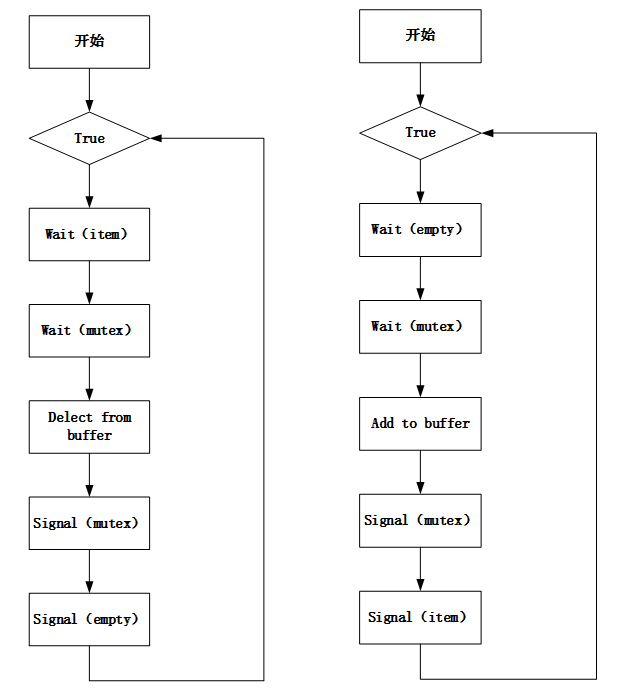
\includegraphics[width=12cm]{f2.png}
	\caption{ 生产者、消费者流程图 \label{fig:1}}
\end{figure}

假设缓冲区大小为10,生产者、消费者线程若干。生产者和消费者相互等效,只要缓冲池未满,生产者便可将消息送入缓冲池;只要缓冲池未空,消费者便可从缓冲池中取走一个消息。我们使用一个互斥量保护生产者向缓冲区中存入数据。由于有多个生产者,因此需要记住现在向缓冲区中存入的位置。使用一个互斥量保护缓冲区中消息的数目,这个生产的数据数目作为生产者和消费者沟通的桥梁。

使用一个条件变量用于唤醒消费者。由于有多个消费者,同样消费者也需要记住每次取的位置。

\subsubsection*{生产者代码块}
\begin{lstlisting}[language=c++]
    void *producer_function(void *args)
    {
        int index = *(int*)args;
        while(1){
            pthread_mutex_lock(&mutex);
            while(g_count >= MAXCAPACITY){
                printf("产品已满,生产者%d等待中\n", index);
                pthread_cond_wait(&condCon, &mutex);
            }
     
            ++g_count;
            printf("生产者%d生产了1个产品,现在共有%d个产品\n", index, g_count);
            pthread_cond_signal(&condPro);
            pthread_mutex_unlock(&mutex);
        }
        pthread_exit(NULL);
    }
\end{lstlisting}

\subsubsection*{消费者代码块}
\begin{lstlisting}[language=c++]
    void *producer_function(void *args)
    {
        int index = *(int*)args;
        while(1){
            pthread_mutex_lock(&mutex);
            while(g_count >= MAXCAPACITY){
                printf("产品已满,生产者%d等待中\n", index);
                pthread_cond_wait(&condCon, &mutex);
            }
     
            ++g_count;
            printf("生产者%d生产了1个产品,现在共有%d个产品\n", index, g_count);
            pthread_cond_signal(&condPro);
            pthread_mutex_unlock(&mutex);
        }
        pthread_exit(NULL);
    }
\end{lstlisting}

在流程图中,两个wait()的顺序是不能调换的。如果调换语句顺序,在生产者发出signal信号后,如果生产者再次获得运行机会,执行完了wait。与此同时一个消费者也执行了wait,但是如果此时缓冲区为空,那么消费者将会发生阻塞,然后生产者也因为无法获得锁而导致阻塞,从而引起死锁。

在程序中,出现了流程不存在的一个额外的while循环。这是为了防止出现假死现象,即唤醒的是同类线程。假设当前多个生产者线程会调用wait方法阻塞等待,当其中的生产者线程获取到对象锁之后通知处于WAITTING状态的线程,如果唤醒的仍然是生产者线程,就会造成所有的生产者线程都处于等待状态。所以程序中添加一个while循环来防止假死的产生。

在程序中还可以看到,互斥锁和条件变量的顺序并不和流程图中的相同。在代码实现中,先添加的互斥锁,再进行wait()的循环。

原因如下,在流程图中的wait()、signal()操作实质上就是操作系统中的PV操作,根据PV操作的定义,该操作语句是原子操作。不会因多线程同时访问共享资源而造成混乱,所以在程序中为了保证线程之间的同步,需要先添加条件变量,然后才进行线程相应的操作,此时互斥锁的作用也是保证共享资源不会被其他线程访问。由于互斥锁的存在,顺序的改变也不会造成死锁的现象。

\section{运行结果}

\begin{figure}[H]
	\centering
	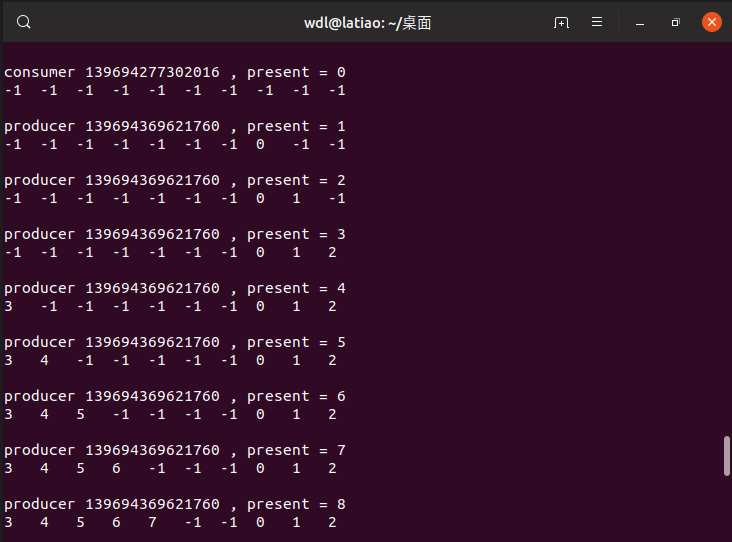
\includegraphics[width=12cm]{f1.png}
	\caption{ 运行结果 \label{fig:1}}
\end{figure}

\section{课程总结}
本次实验学习了设计到在linux系统上多个c++文件的编译,因此学习了如何
使用makefile编写多个c++文件。

这次的课程设计,主要深入理解了关于生产者消费者问题之间互斥和同步的问题,虽然在课堂上已经理解了生产者消费者问题的原理和解决思想,但是在这次的实践中才发现了许多课堂上没有思考到的问题,比如前面提到的假死,还有互斥锁如何使用。在这次课程设计中,我意识到了从理解的原理到实际代码的编写,需要考虑很多现实的问题,从原理到现实的转换是需要付出很多的。生产者消费者问题,其实就是一种有限缓存问题。在缓存区有限的情况下如何进行分配,如何防止死锁的发生。而且由于是在Linux系统上进行的操作,我对Linux系统的操作熟练度也越发提高,也渐渐了解到了Linux系统受编程者欢迎的原因。总的来说这次课程设计收获很多,我的编程水平得到了提高。

% \newpage
% % 代码附录
\begin{appendices}
\section{实验一:彩色图像修复}
\begin{lstlisting}[language=python]
   
\end{lstlisting}
\end{appendices}
%参考文献
\begin{thebibliography}{9}%宽度9
    \bibitem[1]{1}
    李洁, 张瑜慧. 信号量在生产者-消费者及其变形问题中的应用[J]. 福建电脑, 2012(02):175-177.
    \bibitem[2]{2}
    李志民, 赵一丁, 底恒. 操作系统进程同步的教学实践[C]// 计算机研究新进展(2010)——河南省计算机学会2010年学术年会论文集. 2010.步的教学实践[C]计算机研究新进展(2010)——河南省计算机学会2010年学术年会论文集. 2010.
    \bibitem[3]{3}
    陈涛,任海兰. 基于Linux的多线程池并发Web服务器设计[J]. 电子设计工程, 2015(11):175-177.
    \bibitem[4]{4}
    李盼盼, 赵浩. 基于信号量机制的生产者消费者问题的分析[J]. 无线互联科技, 2013(11):101-102.
\end{thebibliography}

% 页尾
\newpage
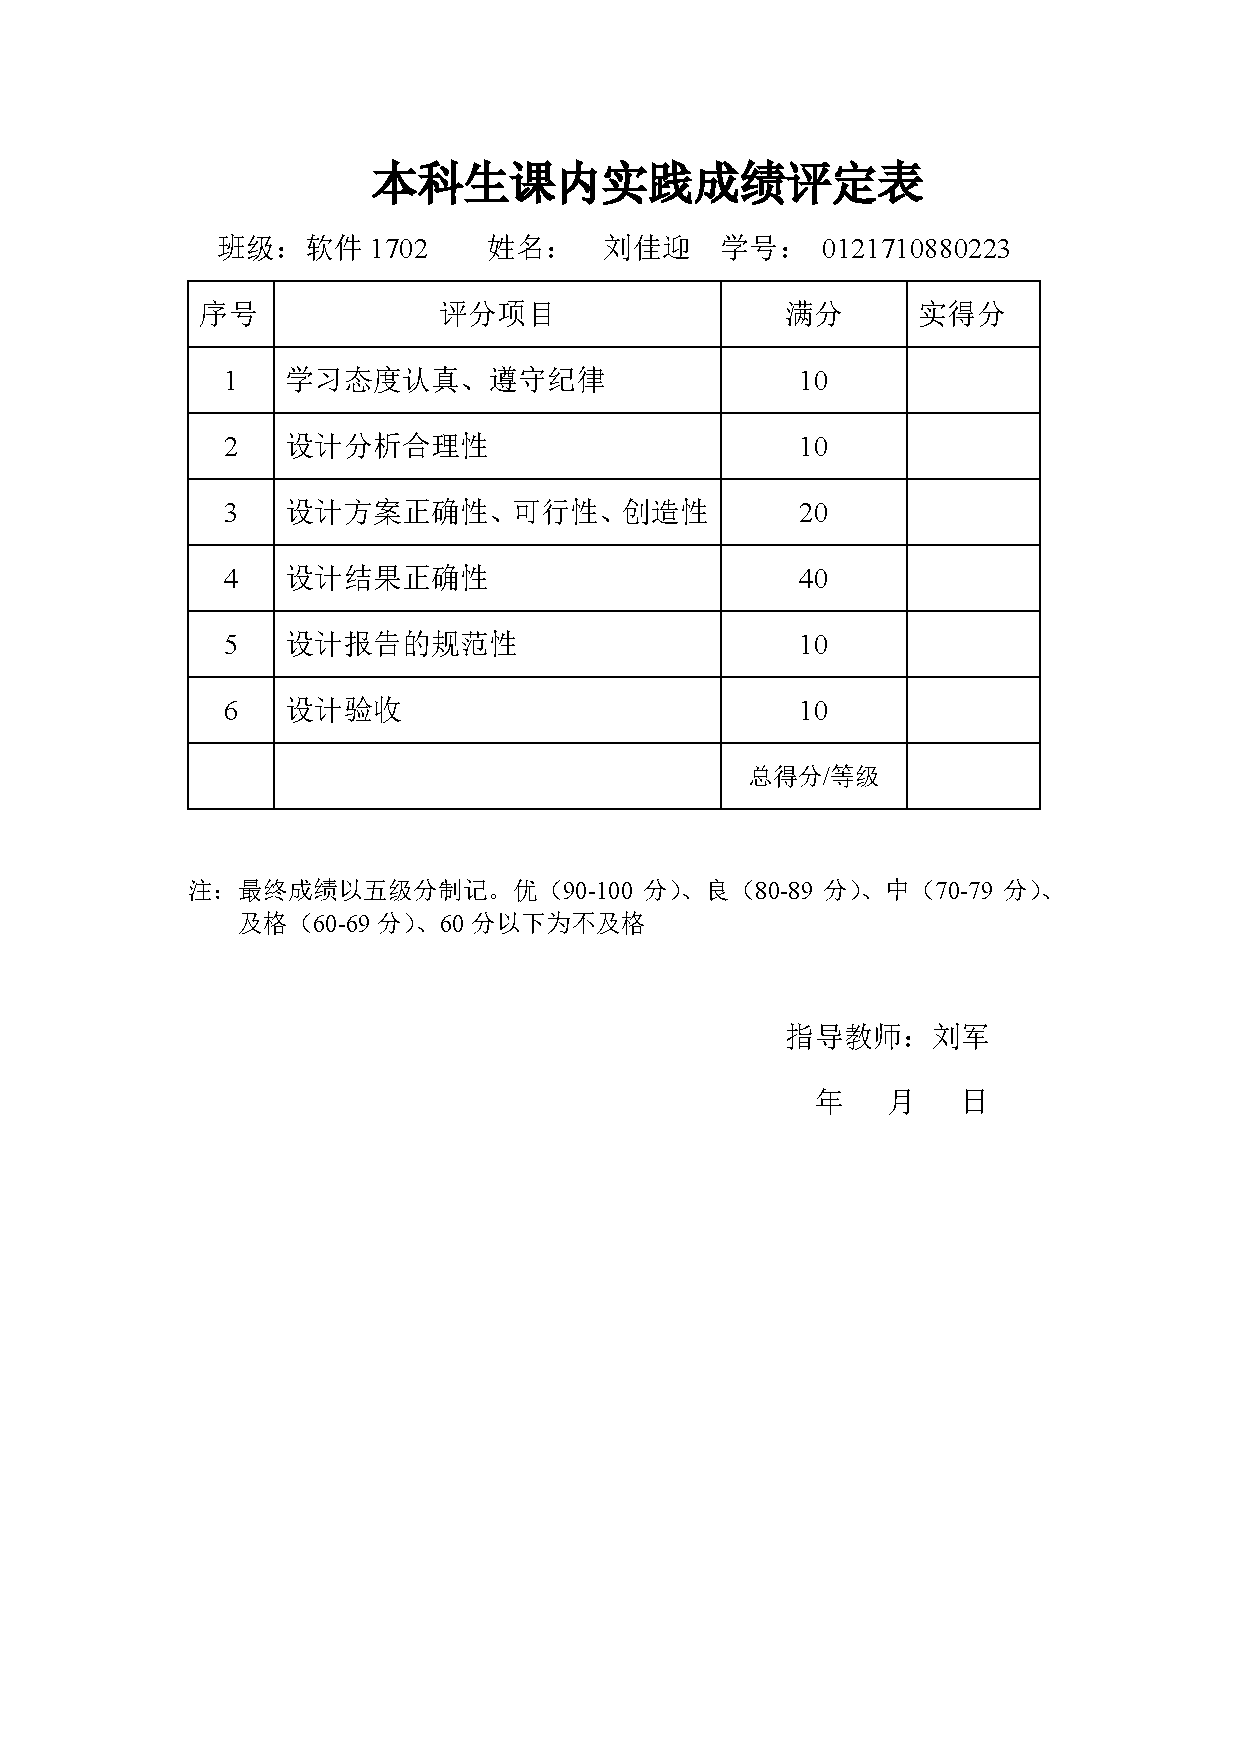
\includepdf[pages={1}]{tag.pdf} 

\end{document}
